\documentclass{beamer}
\usepackage{textcomp}
\usepackage{caption}
\usepackage{listings}

\usetheme{default}

\usebackgroundtemplate{
\includegraphics[width=\paperwidth]{../cpeb_bkground_topleft.pdf}}

\setbeamertemplate{frametitle}[default][center]
  \title{How we do GBS\ldots}
  \subtitle{And what's next?}
  \author{Kevin Murray\\\tiny{\texttt{@kdmurray91}\\kevin@kdmurray.id.au}}
  \institute{Borevitz Lab, ANU}
  \date{MapNet GBS workshop\\23 Oct 2014}

\begin{document}
{
\usebackgroundtemplate{
\includegraphics[width=\paperwidth]{../cpeb_bkground_centered.pdf}}
\begin{frame}
  \titlepage
  \vfill
\end{frame}
}

\begin{frame}{About Me}
  \begin{itemize}
    \item Bioinformatics RA
    \begin{itemize}
      \item TraitCapture Project Developer
      \item Genomics (Low level sequence analysis)
      \item Phenomics (Image analysis)
      \item Sample tracking, data standards, HPC
    \end{itemize}
    \item Starting PhD in Bioinformatics of Evolutionary Genomics next
      year
    \item \textit{``Data Intensive Biologist''}
    \pause
    \item A \textbf{very} lapsed kiwi (from Napier)
  \end{itemize}
\end{frame}

\begin{frame}{What do we use GBS for?}
  \begin{columns}[c]
    \column{0.4\textwidth}
    \begin{itemize}
      \item Population and Landscape Genomics
      \item Population re-sampling
      \item Genotype verification
      \item Epigenomics - HpaII/MspI
    \end{itemize}
    \column{0.6\textwidth}
    \includegraphics<1>[width=0.8\textwidth]{img/landscape_genomics.png}
    \includegraphics<2>[width=0.7\textwidth]{img/resampling.png}
    \includegraphics<3>[width=0.8\textwidth]{img/expt.png}
  \end{columns}
  \vfill
\end{frame}

\begin{frame}{Library preparation}
  \begin{columns}[b]
    \begin{column}{0.4\textwidth}
      \begin{itemize}
        \item We do all our library prep. in house
        \item Cost $\approx$ \$10/sample including extraction
        \item Done in lots of 96
        \item Semi-automated wet-lab protocol
      \end{itemize}
    \vfill
    \end{column}
    \begin{column}{0.6\textwidth}
      \parbox[c][0.7\textheight][c]{\columnwidth}{
      \includegraphics<1>[width=0.8\textwidth]{img/frosty.png}
      \includegraphics<2>[width=0.8\textwidth]{img/janus.png}
      \includegraphics<3>[width=0.8\textwidth]{img/gx2.png}
    }
    \end{column}
  \end{columns}
\end{frame}

\begin{frame}{Library preparation protocol}
  \begin{columns}[t]
    \column{0.5\textwidth}
    \begin{itemize}
      \item Modified protocol from Elshire et al. (2011)
      \item PE 101bp HiSeq 2500 reads
      \item We use in read barcodes
    \end{itemize}
    \column{0.5\textwidth}
    \begin{itemize}
      \item Sequence 576-1152 samples/lane
      \item Need ``combinatorial'' barcoding (next slide)
    \end{itemize}
  \end{columns}
  \begin{center}
    \parbox[t][0.4\textheight][c]{\columnwidth}{
      \includegraphics<1>[width=0.9\textwidth]{img/GBS1.png}
      \includegraphics<2>[width=0.9\textwidth]{img/GBS2.png}
      \vfill
    }
  \end{center}
\end{frame}

\begin{frame}{Combinatorial Barcoding}
  \begin{columns}[t]
    \column{0.5\textwidth}
    \begin{itemize}
      \item We use dual in read barcodes
      \item Independent barcodes for R1 \& R2
      \item Set of 96x12 = 1152/lane
    \end{itemize}
    \column{0.5\textwidth}
    \begin{itemize}
      \item Must be balanced \& staggered
      \item Hamming distance $>$2
    \end{itemize}
  \end{columns}
  \begin{center}
    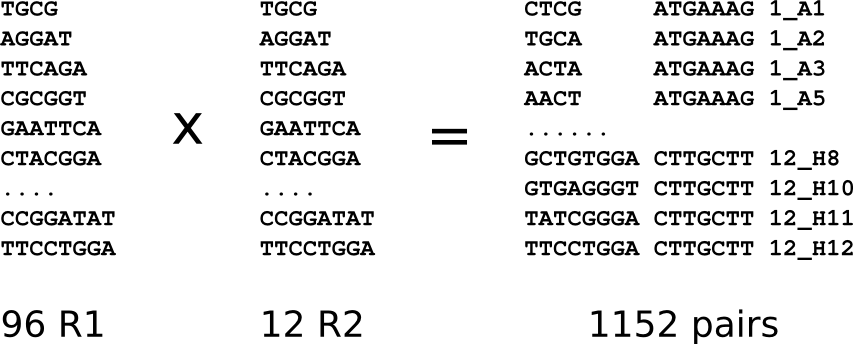
\includegraphics[width=0.8\textwidth]{img/combBcd.png}
  \end{center}
\end{frame}


\begin{frame}{De-multiplex with \texttt{AXE}}
  \begin{columns}[b]
    \column{0.7\textwidth}
    \begin{itemize}
      \item Barcoding scheme requires advanced de-multiplexing
      \item Trie-based lookup algorithm
      \item Fast (PE lane in 5-10 mins)
      \item Highly accurate (99.6\%TPR, 100\%TNR)
      \item Open source at \url{http://git.io/kIhEZA}
      \item Benchmarking IPython notebook at \url{http://bit.ly/1sXrx4E}
    \end{itemize}
    \column{0.3\textwidth}
    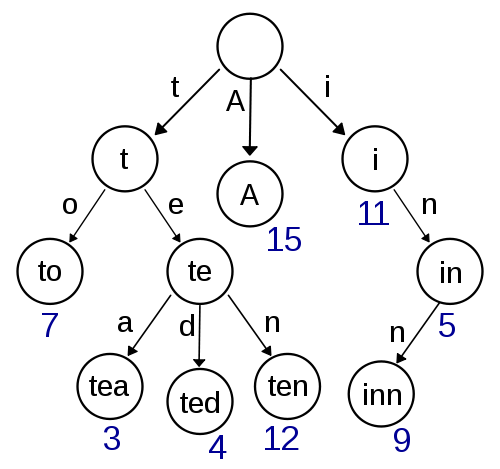
\includegraphics[width=0.8\textwidth]{img/trie.png}
  \end{columns}
  \vfill
\end{frame}

\begin{frame}{Sample Management}
  \begin{itemize}
    \item Sample-tracking system manages FASTQs after demux:
    \begin{itemize}
      \item QC reads (scythe, sickle, seqqs)
      \item After QC, 16-mer globally unique ID re-added to reads
      \item Auto-creates TASSEL KeyFile \& working dir for new analysis
      \item Auto-remove 16-mer unique ID from reads if not using TASSEL.
    \end{itemize}
  \end{itemize}
  \pause
  \begin{itemize}
    \item DB links FASTQs to real world
      \begin{itemize}
        \item Integrate w/ ALA
        \item Provide user-friendly names to downstream analysis
      \end{itemize}
  \end{itemize}
  \vfill
\end{frame}

\begin{frame}{Downstream Analysis}
  \begin{columns}
    \column{0.5\textwidth}
      \begin{minipage}[t][0.7\textheight][t]{\textwidth}
        \begin{itemize}
        \visible<1->{
            \item Variant calling:
            \begin{itemize}
              \item TASSEL!!
              \item We use UNEAK mostly
              \item Ref-based pipeline w/ BWA-MEM
            \end{itemize}
        }
        \visible<2->{
          \item Post analysis in R
          \begin{itemize}
            \item Custom filtering for missing data/paralogy
            \item H-Clust
          \end{itemize}
        }
        \visible<3>{
          \item Downstream:
            \begin{itemize}
              \item Structure
              \item BayENV
              \item QTLRel
            \end{itemize}
        }
        \end{itemize}
      \end{minipage}
    \column{0.5\textwidth}
      \includegraphics<1>[width=0.8\textwidth]{img/uneak.png}
      \includegraphics<2>[width=0.7\textwidth]{img/bd2346.png}
      \includegraphics<3>[width=0.8\textwidth]{img/manhattan.png}
      \vfill
  \end{columns}
\end{frame}

\begin{frame}{The Future!}
  \begin{minipage}[b][0.4\textheight][t]{\textwidth}
    \begin{columns}[b]
      \column{0.5\textwidth}
      \begin{itemize}
        \item<1-3> Better adaptors
        \only<2-3>{
          \item Home-brew NexTera
          \begin{itemize}
            \item NextRAD
            \item Low coverage WGS
            \item Long Pseudo-reads
          \end{itemize}
        }
      \end{itemize}
      \column{0.5\textwidth}
      \only<3>{
        \begin{itemize}
          \item Informatics:
          \begin{itemize}
            \item Imputation?
            \item Paralog/Ploidy detection
            \item Streaming Variant Calling \small{(my PhD)}
          \end{itemize}
        \end{itemize}
      }
    \end{columns}
  \end{minipage}
  \begin{center}
    \includegraphics<1>[width=0.8\textwidth]{img/GBSbetter.png}
    \includegraphics<2>[width=0.8\textwidth]{img/NextRad.png}
    \includegraphics<3>[width=0.8\textwidth]{img/GBSbetter.png}
  \end{center}
  \vfill
\end{frame}

\begin{frame}{Thanks}
  \begin{columns}
    \column{0.5\textwidth}
    \begin{itemize}
      \item Justin Borevitz
      \item Comrades in Informatics
      \begin{itemize}
        \item Aaron Chuah
        \item Riyan Chen
        \item Jared Streich
      \end{itemize}
    \end{itemize}
    \column{0.5\textwidth}
    \begin{itemize}
      \item Wet-lab Wizardry
      \begin{itemize}
        \item Niccy Aitken
        \item Norman Warthmann
      \end{itemize}
    \item Rob for the invitation
    \item You all for listening!!
    \end{itemize}
  \end{columns}
  \vfill
  \begin{columns}
    \column{0.6\textwidth}
    \centering
    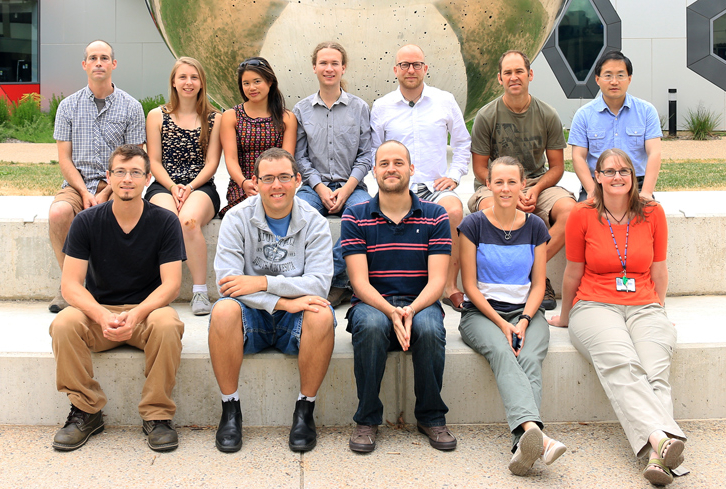
\includegraphics[width=\textwidth]{img/lab.jpg}
    \column{0.3\textwidth}
    \centering
    
\includegraphics[width=\textwidth]{img/qrlink.png}\\
    \small{\url{git.io/TYrIFw}}
    \vfill
  \end{columns}
\end{frame}

\end{document}
